\subsection{The Capital Structure Question and the Pie Theory}
\begin{frame}{Capital Structure and the Pie Theory}
	
	\begin{block}{Firm Value Identity}
		The total value of the firm is the sum of its debt and equity:
		\begin{equation}
			V = B + S
		\end{equation}
	\end{block}
	
	\vspace{-0.3cm}
	\begin{columns}[T]
		\column{0.7\textwidth}
		\textbf{Key Question:}  
		\begin{itemize}
			\item Can the firm change its value by adjusting the mix between debt and equity?
			\item If so, what is the optimal capital structure that maximizes firm value?
			\item This is the \textbf{Capital Structure Question}.
		\end{itemize}
		
		\column{0.3\textwidth}
		\begin{figure}
			\centering
			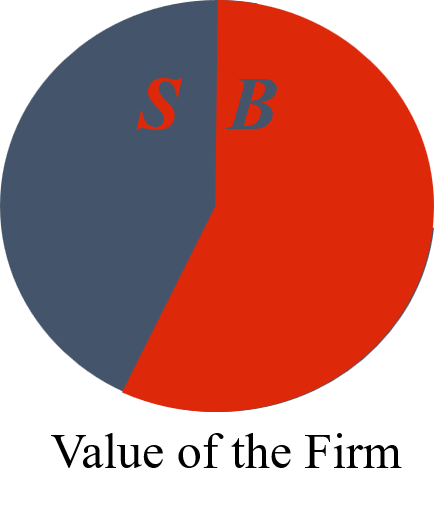
\includegraphics[width=0.6\linewidth]{images/section2/firmvalue}
			\caption*{\tiny Capital structure changes the “slices” -- but does it grow the pie?}
		\end{figure}
	\end{columns}
	
	\vspace{-0.3cm}
	\begin{alertblock}{Objective}
		Choose the debt–equity ratio that \textbf{maximizes the total firm value}.
	\end{alertblock}
	
\end{frame}

\begin{frame}{Stockholders and Capital Structure Decisions}
	
	\textbf{Two Key Questions in Capital Structure:}
	\begin{enumerate}
		\item Why should shareholders care about \textit{maximizing firm value}, rather than just \textit{their own claims}?
		\item What debt–equity ratio maximizes shareholder wealth?
	\end{enumerate}
	
	\vspace{0.5cm}
	\begin{itemize}
		\item A change in capital structure affects the allocation between debt and equity.
		\item But it benefits shareholders \textbf{only if it increases total firm value}.
	\end{itemize}
	
	\vspace{0.3cm}
	\begin{alertblock}{Implication}
		Capital structure is irrelevant to shareholders unless it expands the overall size of the pie.
	\end{alertblock}
	
\end{frame}

\subsection{Financial Leverage and Firm Value: An Example}
\begin{frame}{Leverage Recapitalization: Setup}
	
	\textbf{Trans Am Corporation is currently unlevered.}  
	It is considering issuing \$4,000 of debt to repurchase equity.
	
	\begin{table}[h]
		\centering
		\resizebox{0.9\linewidth}{!}{
			\begin{tabular}{@{}lrr@{}}
				\toprule
				& \textbf{Unlevered} & \textbf{Levered (Proposed)} \\ \midrule
				Total Assets              & \$8,000            & \$8,000                      \\
				Debt                      & \$0                & \$4,000                      \\
				Equity                    & \$8,000            & \$4,000                      \\
				Interest Rate             & 10\%               & 10\%                         \\
				Market Price per Share    & \$20               & \$20                         \\
				Shares Outstanding        & 400                & 200                          \\
				\bottomrule
			\end{tabular}
		}
	\end{table}
	

	\begin{alertblock}{Key Question}
		How does leverage affect EPS and ROE under different operating scenarios?
	\end{alertblock}
\end{frame}

\begin{frame}{EPS and ROE Under Different Scenarios}
	
	\textbf{Unlevered Structure (All-Equity)}
	\begin{table}
		\centering
		\resizebox{0.6\linewidth}{!}{
		\begin{tabular}{@{}lccc@{}}
			\toprule
			& Recession & Expected & Expansion \\ \midrule
			Earnings      & \$400     & \$1,200  & \$2,000   \\
			ROE           & 5\%       & 15\%     & 25\%      \\
			EPS           & \$1       & \$3      & \$5       \\ \bottomrule
		\end{tabular}
	}
	\end{table}
	
	\textbf{Leveraged Structure (Debt = \$4,000)}
	\begin{table}
		\centering
		\resizebox{0.6\linewidth}{!}{
		\begin{tabular}{@{}lccc@{}}
			\toprule
			& Recession & Expected & Expansion \\ \midrule
			EBIT                  & \$400     & \$1,200  & \$2,000   \\
			Interest Expense      & \$400     & \$400    & \$400     \\
			Earnings After Interest & \$0     & \$800    & \$1,600   \\
			ROE                   & 0\%       & 20\%     & 40\%      \\
			EPS                   & \$0       & \$4      & \$8       \\ \bottomrule
		\end{tabular}
	}
	\end{table}
	
	\begin{block}{Observation}
		Leverage increases return sensitivity -- it amplifies both gains and losses.
	\end{block}
	
\end{frame}

\begin{frame}{EPS as a Function of EBIT (Leveraged vs. Unleveraged)}
	
	\begin{figure}
		\centering
		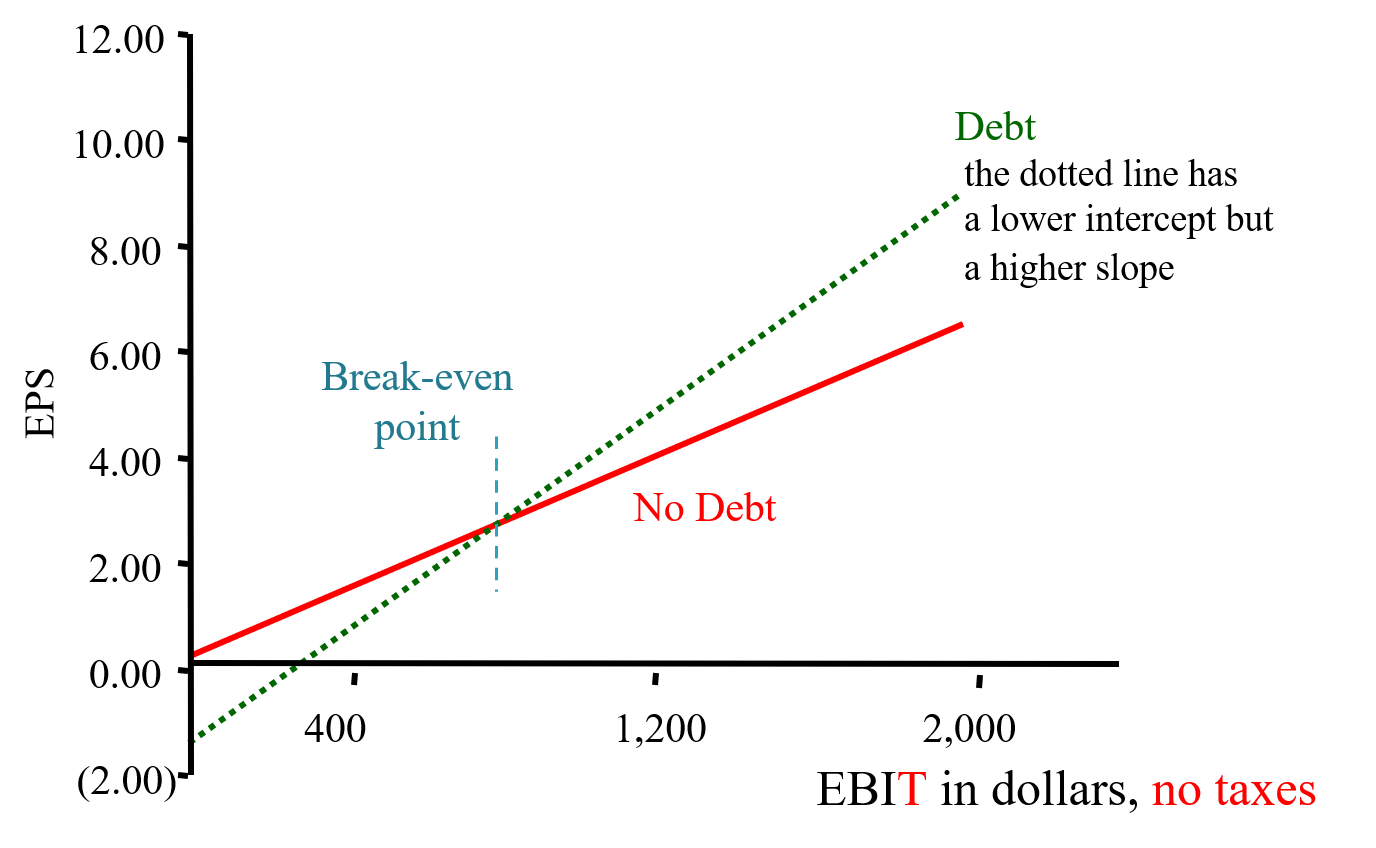
\includegraphics[width=0.6\linewidth]{images/section2/epschanges.png}
	\end{figure}
	
	\vspace{0.3cm}
	\begin{block}{Interpretation}
		The break-even EBIT is where both structures yield the same EPS.  
		Beyond that point, leverage boosts EPS; below it, leverage hurts.
	\end{block}
\end{frame}

\begin{frame}{Break-Even EBIT: When Does Leverage Help?}
	
	\begin{itemize}
		\item Financial leverage increases EPS only when EBIT exceeds a certain threshold -- the \textbf{break-even EBIT}.
		\item Below that point, interest expense outweighs the benefit of fewer shares outstanding.
	\end{itemize}
	
	\begin{block}{Example Setup}
		MPD Corporation plans to shift from an all-equity structure to a leveraged one by issuing \$1 million of debt at 9\% interest to repurchase shares.  
		\vspace{1mm}
		
		Currently:  
		\begin{itemize}
			\item 200,000 shares at \$20/share  
			\item No debt  
		\end{itemize}
		
		\textbf{Question:}  
		What is the minimum EBIT that would make the restructuring EPS-neutral (i.e., the break-even point)?
	\end{block}
	
\end{frame}

\begin{frame}{Break-Even EBIT: Step-by-Step Calculation}
	\small
	\textbf{Unlevered EPS (original):}
	\[
	\text{EPS}_\text{Old} = \frac{\text{EBIT}}{200{,}000}
	\]
	
	\textbf{Leveraged EPS (new):}
	\begin{itemize}
		\item Interest expense = \$1,000,000 × 9\% = \$90,000
		\item Shares repurchased = \$1,000,000 / \$20 = 50,000
		\item Shares outstanding after repurchase = 150,000
		\[
		\text{EPS}_\text{New} = \frac{\text{EBIT} - 90{,}000}{150{,}000}
		\]
	\end{itemize}
	

	\textbf{Set equal:}
	\begin{align*}
		\frac{\text{EBIT}}{200{,}000} = \frac{\text{EBIT} - 90{,}000}{150{,}000} 
		\Rightarrow \text{EBIT} = \$360{,}000
	\end{align*}
	\vspace{-0.4cm}
	\begin{alertblock}{Result}
		EBIT must exceed \$360,000 for leverage to increase EPS.
	\end{alertblock}
	
\end{frame}

\begin{frame}{Interpreting Break-Even EBIT}
	
	\begin{itemize}
		\item \textbf{Definition:}  
		Break-even EBIT is the level at which EPS under two capital structures (leveraged and unleveraged) is equal.
		
		\item \textbf{If EBIT > Break-even:}  
		\begin{itemize}
			\item Leverage amplifies returns (higher EPS)
			\item Financial structure becomes \textbf{advantageous}
		\end{itemize}
		
		\item \textbf{If EBIT < Break-even:}  
		\begin{itemize}
			\item Interest costs drag down earnings
			\item Leverage is \textbf{detrimental} -- equity returns shrink, risk of distress rises
		\end{itemize}
		
		\item \textbf{Managerial Use:}  
		Helps determine when adding leverage is expected to create or destroy shareholder value
	\end{itemize}
	
	\begin{block}{Teaching Insight}
		Break-even EBIT offers a bridge between capital structure theory and real-world decision-making.
	\end{block}
	
\end{frame}

\begin{frame}{Homemade Leverage: Core Insights}
	
	\begin{itemize}
		\item \textbf{Key Idea:}  
		Investors can replicate the effects of corporate leverage by borrowing on their own account.
		
		\item \textbf{Implications from Example:}
		\begin{itemize}
			\item At high EBIT levels, leverage magnifies shareholder returns (EPS, ROE $\uparrow$).
			\item At low EBIT levels, fixed interest costs amplify downside risk (EPS, ROE $\downarrow$).
			\item Financial leverage increases the volatility of shareholder outcomes.
			\item Because investors can replicate leverage on their own, capital structure may be irrelevant -- under ideal conditions.
		\end{itemize}
	\end{itemize}
	
	\vspace{0.2cm}
	\begin{alertblock}{Takeaway}
		The value of the firm should not depend on how it's financed -- if investors can create “homemade leverage.”
	\end{alertblock}
	
\end{frame}

\begin{frame}{Comparing Corporate and Homemade Leverage}
	\vspace{-0.2cm}
	\begin{table}[h]
		\centering
		\resizebox{0.9\linewidth}{!}{
			\begin{tabular}{@{}lccc@{}}
				\toprule
				\textbf{Scenario} & \textbf{Recession} & \textbf{Expected} & \textbf{Expansion} \\
				\midrule
				\multicolumn{4}{l}{\textit{Strategy A: 100 Shares of Levered Equity}} \\
				EPS (Levered)     & 0    & \$4   & \$8   \\
				Total Earnings    & 0    & \$400 & \$800 \\
				Initial Investment & \multicolumn{3}{r}{100 × \$20 = \$2,000} \\
				\midrule
				\multicolumn{4}{l}{\textit{Strategy B: Homemade Leverage (200 Unlevered – \$2,000 borrowed)}} \\
				EPS (Unlevered)   & \$1   & \$3   & \$5   \\
				Total Earnings    & \$200 & \$600 & \$1,000 \\
				Interest Expense  & \$200 & \$200 & \$200 \\
				Net Earnings      & 0     & \$400 & \$800 \\
				Initial Investment & \multicolumn{3}{r}{200 × \$20 – \$2,000 = \$2,000} \\
				\bottomrule
			\end{tabular}
		}
	\end{table}
	
	\begin{block}{Conclusion}
		Investor-created leverage perfectly replicates corporate leverage -- under ideal conditions.
	\end{block}
	
\end{frame}

\begin{frame}{What Does Homemade Leverage Teach Us?}
	
	\begin{itemize}
		\item \textbf{If} investors can borrow and lend at the same rate as firms,  
		\item \textbf{And if} there are no taxes, transaction costs, or bankruptcy costs,
	\end{itemize}
	
	\vspace{0.3cm}
	\begin{block}{Then...}
		Capital structure becomes irrelevant:  
		\[
		\text{Firm Value (V)} \quad \text{is the same whether it’s financed by debt or equity.}
		\]
	\end{block}
	
	\vspace{0.2cm}
	\begin{itemize}
		\item Investors can always adjust leverage themselves.
		\item This logic forms the foundation of the \textbf{Modigliani–Miller Proposition I}.
	\end{itemize}
\end{frame}

\subsection{Modigliani–Miller Model}
\begin{frame}{Capital Structure: Does It Matter?}
	
	\begin{itemize}
		\item In 1958, \textcite{modigliani1958cost} proposed a revolutionary theory of capital structure.  
		\item Their core question: \textbf{Can financing choices affect firm value?}
		\item The M\&M model provides a framework to explore when capital structure is irrelevant -- and when it matters.
	\end{itemize}
	
	
	\vspace{0.2cm}
	\begin{alertblock}{What Comes Next}
		We will analyze three progressively more realistic cases that relax ideal assumptions.
	\end{alertblock}
	
\end{frame}

\begin{frame}{Three Cases in M\&M Capital Structure Theory}
	
	\begin{itemize}
		\item \textbf{Case I: Perfect Capital Markets}
		\begin{itemize}
			\item No taxes, no transaction costs, no bankruptcy
			\item Capital structure is irrelevant
		\end{itemize}
		
		\item \textbf{Case II: Corporate Taxes Introduced}
		\begin{itemize}
			\item Interest is tax-deductible $\rightarrow$ Debt creates value
			\item Incentive to fully lever up
		\end{itemize}
		
		\item \textbf{Case III: Taxes + Financial Distress}
		\begin{itemize}
			\item Trade-off between tax shield and bankruptcy risk
			\item Optimal capital structure balances both
		\end{itemize}
	\end{itemize}
	
	\vspace{0.2cm}
	\begin{block}{Literature Evolution}
		These cases laid the foundation for the \textit{trade-off theory} of capital structure.  
		See also: \textcite{miller1988nobel}
	\end{block}
	
\end{frame}
\begin{frame}{Key Assumptions Behind the M\&M Model}
	
	\textbf{To understand why capital structure may be irrelevant, we must first understand the model’s ideal conditions:}
	
	\vspace{0.3cm}
	\begin{itemize}
		\item \textbf{Perfect Capital Markets}
		\begin{itemize}
			\item No taxes or transaction costs
			\item Firms and investors borrow/lend at the same rate
			\item No asymmetric information
		\end{itemize}
		
		\item \textbf{Homogeneous Expectations}
		\begin{itemize}
			\item All investors agree on firm cash flows and risk
		\end{itemize}
		
		\item \textbf{Same Risk Class}
		\begin{itemize}
			\item Firms compared must have similar business risk
		\end{itemize}
	\end{itemize}
	
	\vspace{0.2cm}
	\begin{alertblock}{Next}
		We now turn to Case I -- where capital structure does not affect firm value.
	\end{alertblock}
	
\end{frame}

\subsubsection{Case I}
\begin{frame}{MM Proposition I (No Taxes): Value Irrelevance}
	
	\begin{block}{M\&M Proposition I}
		Under perfect capital markets and no taxes:
		\[
		V_L = V_U
		\]
		\textit{The value of a levered firm equals that of an unlevered firm.}
	\end{block}
	
	\begin{itemize}
		\item Firm value is determined solely by the cash flows and risk of its assets.
		\item Capital structure does not create or destroy value -- it’s just slicing the same pie differently.
		\item Investors can replicate any capital structure through homemade leverage.
	\end{itemize}
	
	\vspace{0.2cm}
	\tiny{\textcite{modigliani1958cost}}
\end{frame}

\begin{frame}{MM Proposition II (No Taxes): Cost of Equity}
	
	\begin{block}{M\&M Proposition II}
		As leverage increases, equity becomes riskier:
		\[
		R_S = R_0 + \frac{B}{S}(R_0 - R_B)
		\]
	\end{block}
	
	\begin{itemize}
		\item \(R_S\): Cost of equity  
		\item \(R_0\): Cost of capital for the unlevered firm (business risk)  
		\item \(R_B\): Cost of debt  
	\end{itemize}
	\begin{exampleblock}{Key Insight:}
		Equity holders demand higher returns as financial leverage increases risk.
	\end{exampleblock}
	
\end{frame}

\begin{frame}{MM Proposition II: Derivation}
	
	\textbf{Start with WACC:}
	\[
	R_0 = \frac{B}{B+S} R_B + \frac{S}{B+S} R_S
	\]
	
	\vspace{0.3cm}
	\textbf{Multiply both sides by } \(\frac{B+S}{S}\):
	
	\[
	\frac{B}{S} R_B + R_S = \frac{B+S}{S} R_0
	\]
	
	\vspace{0.3cm}
	\textbf{Solve for } \(R_S\):
	
	\[
	R_S = R_0 + \frac{B}{S}(R_0 - R_B)
	\]
	
	\begin{block}{Conclusion}
		Equity return increases linearly with the debt-equity ratio.
	\end{block}
	
\end{frame}

\begin{frame}{Visualizing Leverage and the Cost of Capital}
	\vspace{-0.5cm}
	\begin{figure}
		\centering
		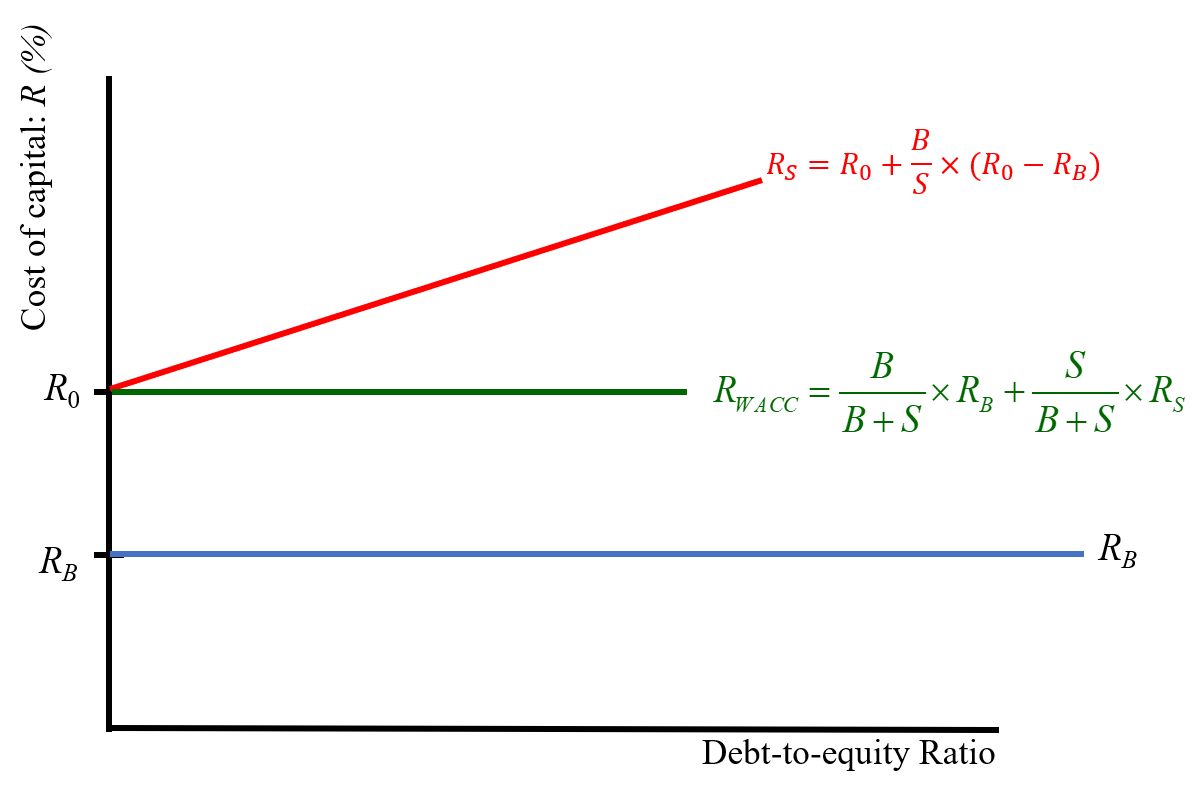
\includegraphics[width=0.7\textwidth]{images/section2/wacc.png}
	\end{figure}
	\vspace{-0.5cm}
	\begin{block}{Interpretation}
		\begin{itemize}
			\item \(R_S\) increases with leverage due to higher risk.
			\item \(WACC = R_0\) remains constant -- consistent with M\&M Proposition I.
		\end{itemize}
	\end{block}

\end{frame}

\begin{frame}{Business Risk vs. Financial Risk}
	
	\textbf{According to M\&M Proposition II:}
	
	\begin{itemize}
		\item The cost of equity includes:
		\begin{enumerate}
			\item \textbf{Business Risk} -- driven by operations and assets.
			\item \textbf{Financial Risk} -- introduced by the use of leverage.
		\end{enumerate}
		
		\item \(R_S = R_0 + \frac{B}{S}(R_0 - R_B)\)
		\begin{itemize}
			\item \(R_0\): captures business risk
			\item \(\frac{B}{S}(R_0 - R_B)\): captures financial risk
		\end{itemize}
		
		\item Leverage does not affect business risk -- only financial risk.
	\end{itemize}
	
	\vspace{0.2cm}
	\begin{alertblock}{Conclusion}
		More leverage $\rightarrow$ more financial risk $\rightarrow$ higher required return on equity.
	\end{alertblock}
	
\end{frame}
